\documentclass[11pt]{article}

%%% Load some useful packages:
%% "New" LaTeX2e graphics support.
\usepackage{graphicx}
%%	using final option to force graphics to be included even in draft mode
%\usepackage[final]{graphicx}

%% Support sub-figures.
\usepackage{subfigure}

%% Make subsubsections numbered and included in ToC
\setcounter{secnumdepth}{3}
\setcounter{tocdepth}{3}

%% Package to linebreak URLs in a sane manner.
\usepackage{url}

%% Define a new 'smallurl' style for the package that will use a smaller font.
\makeatletter
\def\url@smallurlstyle{%
  \@ifundefined{selectfont}{\def\UrlFont{\sf}}{\def\UrlFont{\small\ttfamily}}}
\makeatother
%% Now actually use the newly defined style.
\urlstyle{smallurl}

%% Make margins less ridiculous
\usepackage{fullpage}

%% Allows insertion of fixme notes for future work
\usepackage[footnote, nomargin]{fixme}

%%%% Turned off for tech report, should be turned on for research portfolio
%% Turn on double spacing
%\usepackage{setspace}
%\doublespacing

%% Make URLs clickable
\usepackage[colorlinks, bookmarks=true]{hyperref}
\usepackage[all]{hypcap}


%% Since I'm using the LaTeX Makefile that uses dvips, I need this
%% package to make URLs break nicely
\usepackage{breakurl}

\usepackage{array}

%% Make table cross pages.
\usepackage{longtable}

\begin{document}

\title{Makahiki: A framework for serious games for sustainability\\
\em  A Research White Paper}

\author{
	 Yongwen Xu \\
\em  Collaborative Software Development Laboratory \\
\em  Department of Information and Computer Sciences \\
\em  University of Hawai'i at Manoa\\
     yxu@hawaii.edu \\
}

\date{\today}
\maketitle

\tableofcontents

\graphicspath{{figures/}} 
\DeclareGraphicsExtensions{.eps} 

\newpage
\begin{abstract}

My research seeks to investigate how to build a customizable serious game engine for sustainability called Makahiki. It provides an open source, component-based, extensible framework for creating serious games for the purpose of education and behavioral change regarding energy, water, food, and waste generation and use. Different organizations configures the Makahiki framework to produce a ``challange instance'' with a specific set of game mechanics, user interface features, and experimental goals. Makahiki provides sophisticated instrumentation to support evaluation of how well the game mechanics supported the organization's goals for the challenge.

This white paper describes the Makahiki's research goal, system design, and experimental design on how to evaluate the effectiveness of the Makahiki as framework in developing serious games for sustainability.
\end{abstract}


%% Contains introduction to the related work when used outside the
%% context of the dissertation proposal
\section{Introduction}

Sustainability education and conservation has become an international imperative due to the rising cost of energy, increasing scarcity of natural resources and irresponsible environmental practices. 
Over the past decade, running energy and water challenges have become a focal point for sustainability efforts at university, government, and industry campuses. Designers of those competitions have had three choices for information technology: (a) build their own custom in-house solution; (b) out-source to a commercial provider; or (c) use a "minimal tech" solution such as a web page and manual posting of data and results.

We developed a framework called Makahiki as a new choice: an extensible game engine for the development and evaluation of sustainability challenges. Makahiki has a unique feature set intended to foster more rapid innovation and development. These features include: (1) an open source license and development model which makes the technology available without charge and facilitates collaborative development and improvement; (2) support for an "ecosystem" of extensible, interrelated, customizable games and activities; (3) real-time game analytics and A/B testing for research and evaluation; (4) pedagogically organized and extensible learning activities; (5) a responsive user interface supporting mobile, tablet, and laptop displays; and (6) support for deployment to the cloud as an inexpensive option for hosting the competition.

The Makahiki framework will be used in 2012 by three organizations, namely, University of Hawaii at Manoa, Hawaii Pacific University, East West Center of University of Hawaii, to implement individually tailored sustainability challenges focusing on energy and water conservation. 

\section{Research Goals}

There are two research goals in Makahiki: (a) provides an extensible framework to easily create engaging games for sustainability education and behavior change, and (b) provides an experimental test bed for Gamification research into the effectiveness of different game mechanics in the context of sustainability.

The challenges of creating a customizable game engine are:  (a) creating a new instance of Makahiki by selecting the games they want the system to support, and (b) extending Makahiki by writing new game components, and (c) supporting ease of use by non-technical organizations with minimal technical support.

In order to provide an experimental test bed for game research, Makahiki will be designed to support A-B testing, where different game mechanics could be configured using the game engine to create ``treatments'' for different user groups. The game engine will provide real-time game analytics to these treatments.

\section{System Design}

Makahiki consists of a configurable game engine that can be customized to the needs of
different organizations.  It includes a library of pre-built game ``widgets'' that
implement a variety of game mechanics.  Using the widgets, an organization can create a
custom energy challenge in which players can compete individually and/or in teams to earn
the most points by reducing their energy consumption as well as by learning about energy
concepts in general.

Figure \ref{fig:system-architecture} illustrates
the architecture of Makahiki.

\begin{figure}[htbp] %  figure placement: here, top, bottom, or page
   \centering
   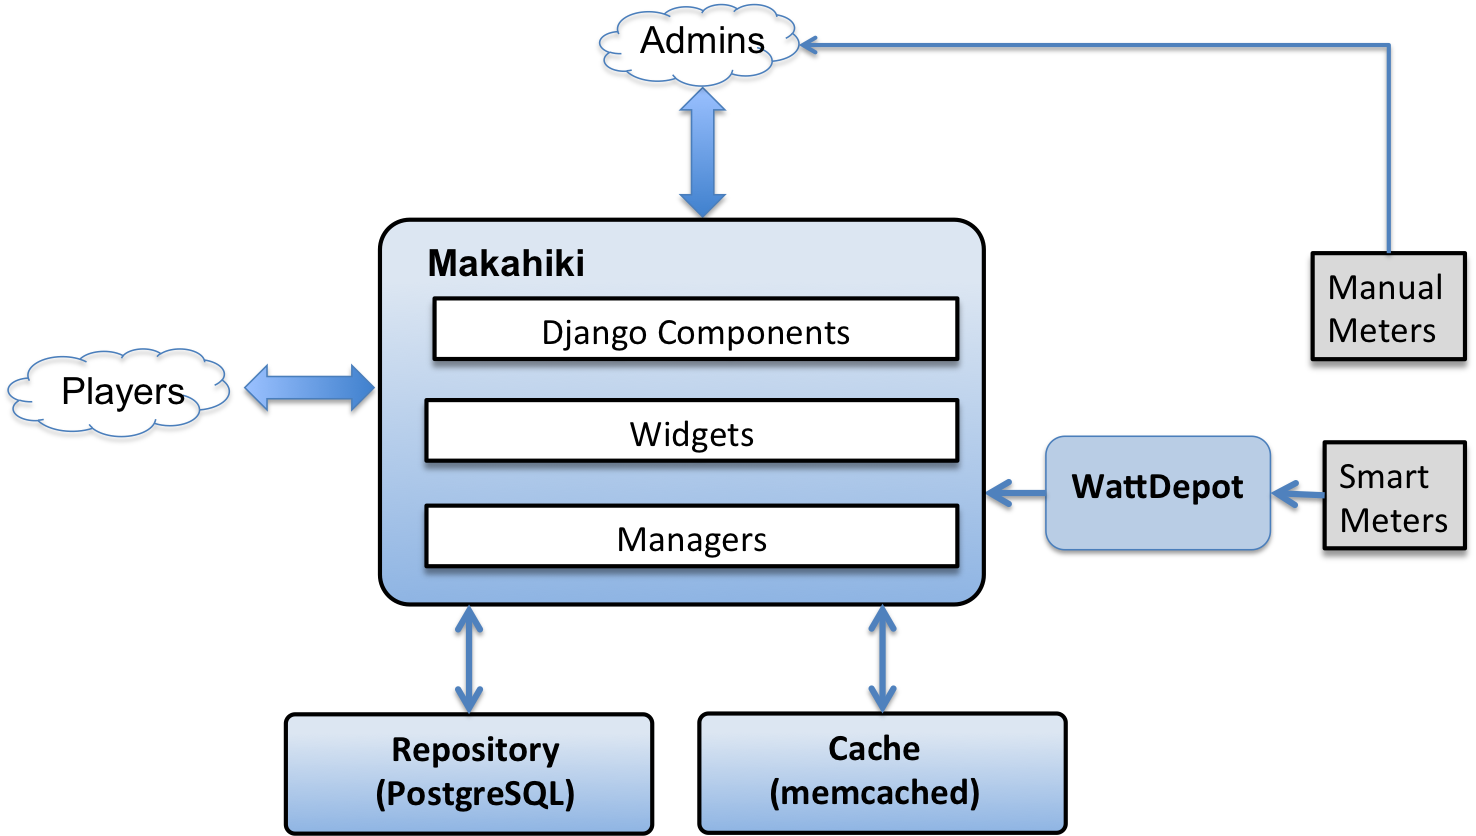
\includegraphics[height=20em]{system-architecture.png} 
   \caption{Makahiki System Architecture}
   \label{fig:system-architecture}
\end{figure}


\section{Experimental Design}

In order to evaluate how the Makahiki meets the research goals, we propose to investigate the following the research questions:

\begin{enumerate}

\em \item Can Makahiki be successfully deployed in multiple organizational scenarios to provide games for major sustainability issues (energy, water, waste, recycling, transportation, etc.)? \em
\em \item Can Makahiki provide an API and procedures to support enhancement with new features and capabilities with a minimum of impact on other aspects of the framework? \em
\em \item Can Makahiki provide an engaging and fun learning user interface to its end users? \em
\em \item Can Makahiki provide a mean to perform research on games for sustainability through A/B testing? \em

\end{enumerate}

\subsection{Site Administration Case Study}
To evaluate question (1), we plan to perform the Site Administration Case Study research on multiple cases. It consists of structured interview process with the site administrators and the correlated data analysis of the archived email changes regarding the administration of the challenges.

\subsubsection{Methodology}

We plan to perform structured interviews to the site administrators of the HPU and East-West Center Challenges. There are two site administrators for each site: one whose main role is responsible for the system installation, deployment of the application, etc; another whose main role is responsible for the challenge administration, including setting up the users, game settings, prizes, etc.

We will undertake three interviews for each site administrator:
a. Pre-challenge interviews
b. In-challenge interviews
c. Post-challenge interviews
The Pre-challenge interviews happen before the challenge. They evaluate how easy or difficult for a system administrator and challenge administrator to install, setup, configure a challenge tailored to their specific requirements. The In-challenge interviews happen during the challenge. They evaluate the required work for administrating the site during the challenge. The Post-challenge interviews happen after the challenge. They evaluate the overall experience of the site administration.

We will record the structured interviews and archive the email exchanges with the site administrators for correlated data analysis.

\subsubsection{Data Analysis}
We will analyze the following data collected from the interviews and email changes:
\begin{itemize}
 \item time taken to install the Makahiki
 \item time taken to configure the Challenge
 \item number of problems encountered
 \item time taken in training
 \item number of problems encountered in training
 \item time taken in admining the challenge
 \item number of problems encountered during the admining the challenge
\end{itemize}

\subsection{Development Enhancement Case Study}
To evaluate question (2), we plan to perform the Development Enhancement Case Study research on at least one case. It consists of a ``case study'' of an external developer who is tasked with making an enhancement to the system.  The goal for the developer evaluation is to find out: (a) What kinds of learnings must occur, (b) What kind of background is necessary from a developer to enhance the system, (c) What kinds of problems were encountered and how they were resolved, (d) What kinds of changes to the system could be made to address the problems.

\subsubsection{Methodology}
\begin{enumerate}
\item \em Log Book\em: We will create a google Form for the developer to fill out at the end of each programming session. Figure \ref{fig:developer-eval-form} illustrates the google form used for Makahiki developer evaluation.

\begin{figure}[htbp] %  figure placement: here, top, bottom, or page
   \centering
   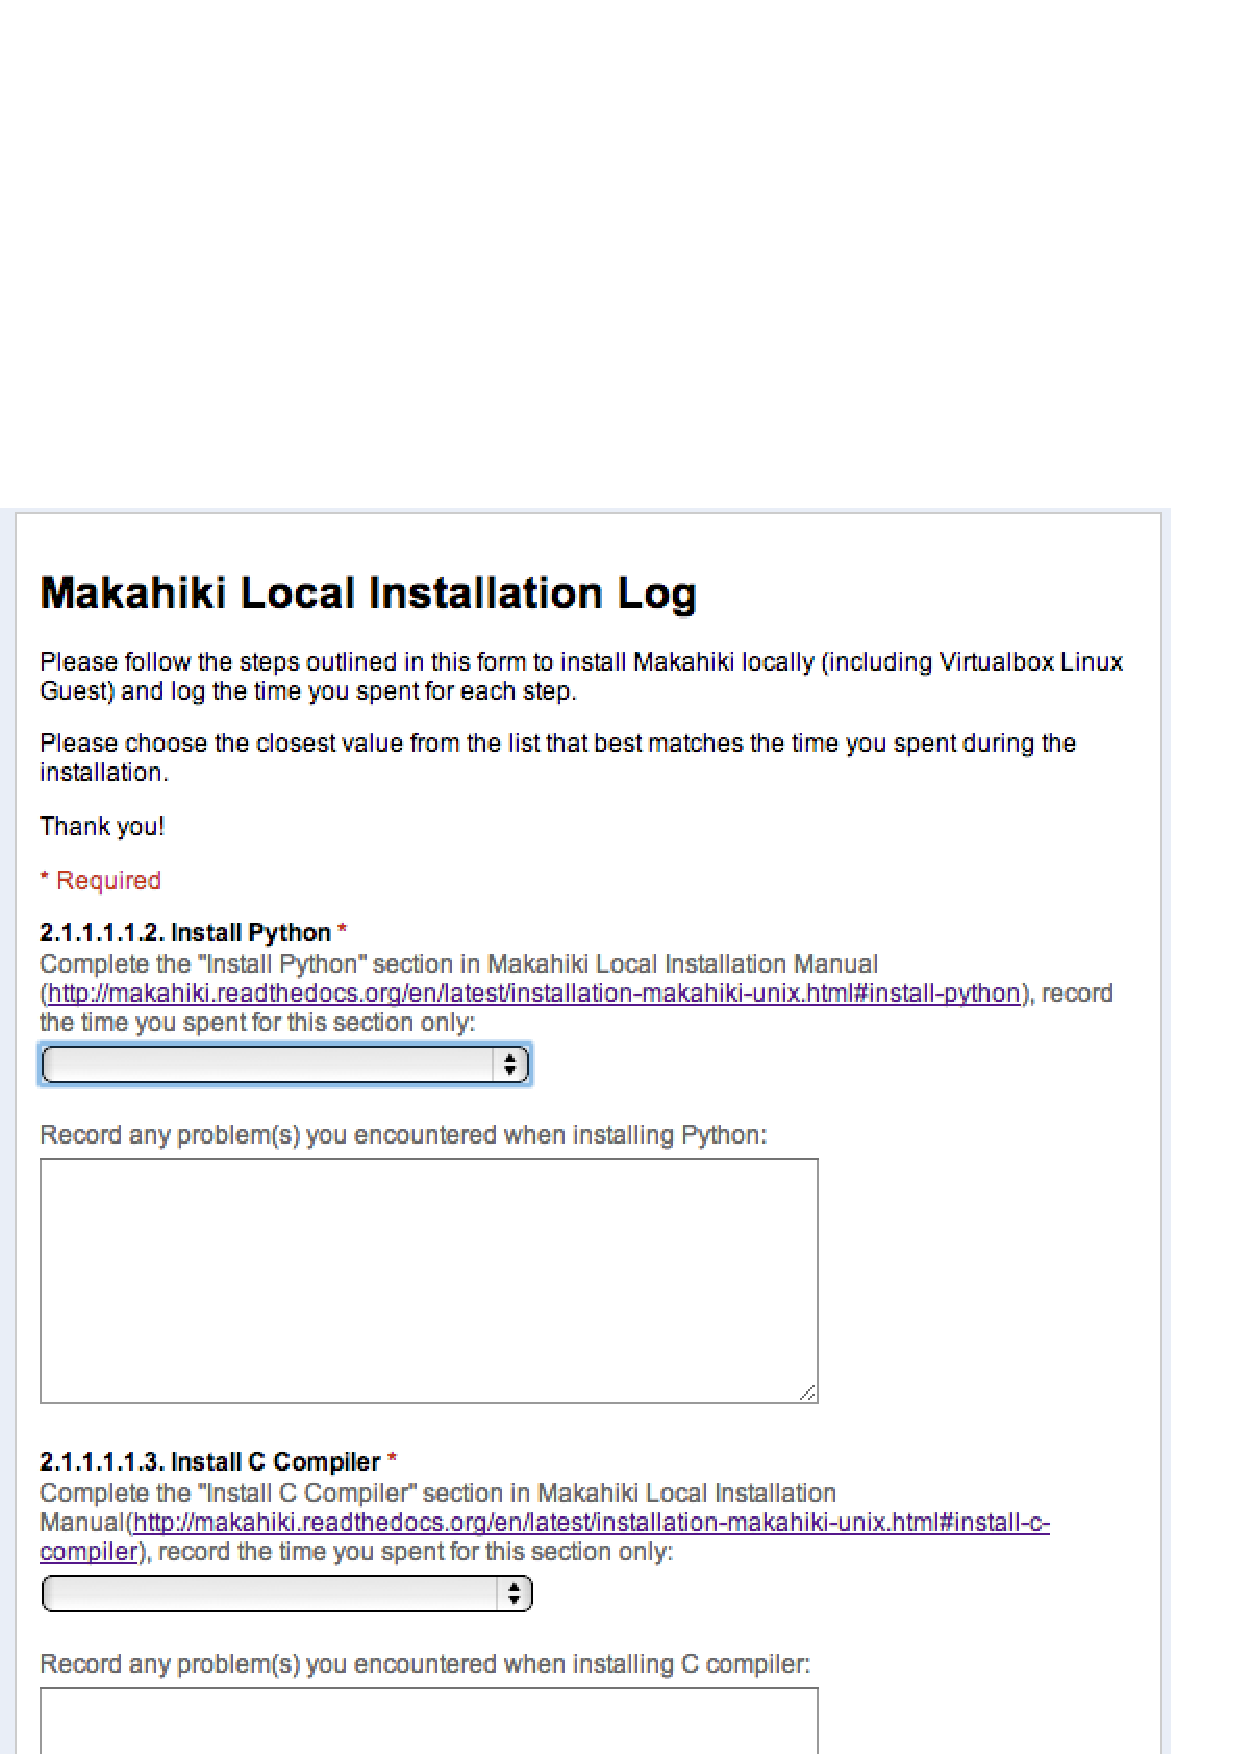
\includegraphics[height=25.5em]{developer-eval-form} 
   \caption{Makahiki Developer Evaluation Form}
   \label{fig:developer-eval-form}
\end{figure}
 
\item \em Meetings \em: We will have weekly developer meetings. we will record the meetings to support the analysis of development usability. we will focus on what kind of problems were encountered during the development.

\item \em Emails and Chat sessions \em: We will save the email exchanges with the developer and the online chat sessions for further analysis.

\end{enumerate}

\subsubsection{Data Analysis}
\begin{itemize}
 \item time taken to setup the development env
 \item number of errors encountered
 \item interactions (emails, chats, meetings) with internal developers
 \item time spent in reading the doc initially
 \item time spent in reading the doc during the development
 \item time taken to create the initial revision of the enhancement
 \item time taken for unit testing, debugging
 \item time taken to integrate into the system
 \item number of makahiki APIs used
 \item metrics of commits, interactions in Github
 
\end{itemize}

\subsection{End User Evaluation}
To evaluate question (3), we plan to perform End User Evaluation with in-game survey and aggregated analytics from the logging data collected from all sites.

\subsubsection{Methodology}

\em In-game surveys \em will be implemented as an activity action in smartgrid game in the challenge. Players can earn points by completing the survey action. 

We plan to collect the logging data from all three sites to assess users' interaction with the system, the reliability and performance of the system.

\subsubsection{Data Analysis}
\begin{itemize}
 \item Popular Quests, Events, Activities, Commitments, RSVPs
 \item Referrals
 \item Daily logins, New Users
 \item Action Feedback
 \item Errors occurred
 \item Numbers of long latency responses
\end{itemize}

\subsection{A/B Testing Evaluation Case Study}
To evaluate question (4), we plan to perform the case study research on at least one case. It consists of a ``case study" of one A/B test from three sites in order to answer the following research question: What level of energy data "latency" is required to provide useful feedback to participants in energy challenges like the Kukui Cup?  To assess this, we will implement three levels of energy latency:  (a) Subminute-level latency through the Power Meter at Hawaii Pacific University site; (b) Hour-level latency through the Daily Energy Goal Game at University of Hawaii site (no Power Meter); and (c) Day-level latency through the manual Daily Energy Goal Game at East West Center site.  In-game surveys will  be used at each site to determine how much participants interacted with the given type of feedback, and whether they felt limited by the given level of latency.

\subsubsection{Methodology}

\subsubsection{Data Collected}
  
%% Use this for an alphabetically organized bibliography
%%\bibliography{sustainability,csdl-trs,gamification}
%%\bibliographystyle{plain}

\end{document}
